

\subsection{Lattice setup}
    Gauge configurations in this work were obtained from the ensemble A40.24 which has been generated using $N_f = 2 + 1 + 1$ quark flavors. Details can be looked up in \cite{guage_configurations}.
    
    \begin{table}[h]
        \centering
        \begin{tabular}{lllllll}
        \hline
        \multicolumn{1}{|c|}{$\#$ used configurations} & \multicolumn{1}{c|}{$\beta$} & \multicolumn{1}{c|}{$\kappa$} & \multicolumn{1}{c|}{$a\mu_I$} & \multicolumn{1}{c|}{$a\mu_\sigma$} & \multicolumn{1}{c|}{$a\mu_\delta$} & \multicolumn{1}{c|}{$(L/a)^3 \times T$} \\ \hline
        \multicolumn{1}{|c|}{11} & \multicolumn{1}{c|}{3.9} & \multicolumn{1}{c|}{0.160856} & \multicolumn{1}{c|}{0.0040} & \multicolumn{1}{c|}{??} & \multicolumn{1}{c|}{??} & \multicolumn{1}{c|}{$24^3 \times 48$} \\ \hline
                               &                       &                       &                       &                       &                       &                       \\
                               &                       &                       &                       &                       &                       &                      
        \end{tabular}
        \caption{Parameters of gauge configurations used}
        \label{table_gauge_params}
    \end{table}
    % TODO explanation
    
\subsection{Meson masses}
    To investigate the accuracy and usefulness of the method of distillation described in this thesis comutations of charmonium state correlation functions where performed. These enable one to test different configurations of eigenvectors in relatively short times compared to the use of light doublet states. Beside the number of gauge configurations the number of eigenvectors can be arbitrarily set. In this section I will present the results for 2, 5 and 10 eigenvectors on the 11 gauge configurations mentioned in the previous section.\\
    
    In all computations the following creation operator was used:
    \begin{equation}
        \Operator(t) = \bar{\chi}^{(c)}(t)\gamma_5\chi^{(c)}(t)
    \end{equation}
    Therefore the resulting meson has quantum numbers $0(0^-)$. This was achieved by using for both propagators $(D^{-1(f)})$ the same flavor $f$. This approach reduced the amount of inversions that had to be calculated significantly. For the same reason a charmonium state was chosen in contrast to e.g. the calculation of a pion mass. Inversion for particles with higher masses converge significantly faster.
    
    To compute the mass of the charmonium state the mean value of all configurations for one value of $\Delta t$ were computed and a simple linear function was fitted to $ln(C(\Delta t))$. The results for 1, 2, 5 and 10 eigenvectors can be seen in figure \ref{1_2_5_10_evs_log}. One can see the similar shapes of all four results. Because the exponential nature of the correlation function only holds for $\Delta t \rightarrow \infty$ only a few points were chosen to be fitted. A more detailed explanation will be presented in the next section.
    
    The masses of these four simulations are:
    \begin{table}[h]
            \centering
            \begin{tabular}{|c|c|}
            \hline
            \multicolumn{1}{|c|}{Number of eigenvectors} & \multicolumn{1}{c|}{Mass (MeV)} \\ \hline
             1 & $3082 \pm 255$\\
             2 & $3227 \pm 215$\\
             5 & 1\\
             10& $2919 \pm 88$\\
              \hline
            \end{tabular}
            \caption{Calculated masses for the charmonium state}
            \label{meson_masses}
        \end{table}
        
    The errors were calculated using the \textit{Jackknife}\cite{jackknife} method.
    
    \begin{figure}[H]
        \centering
        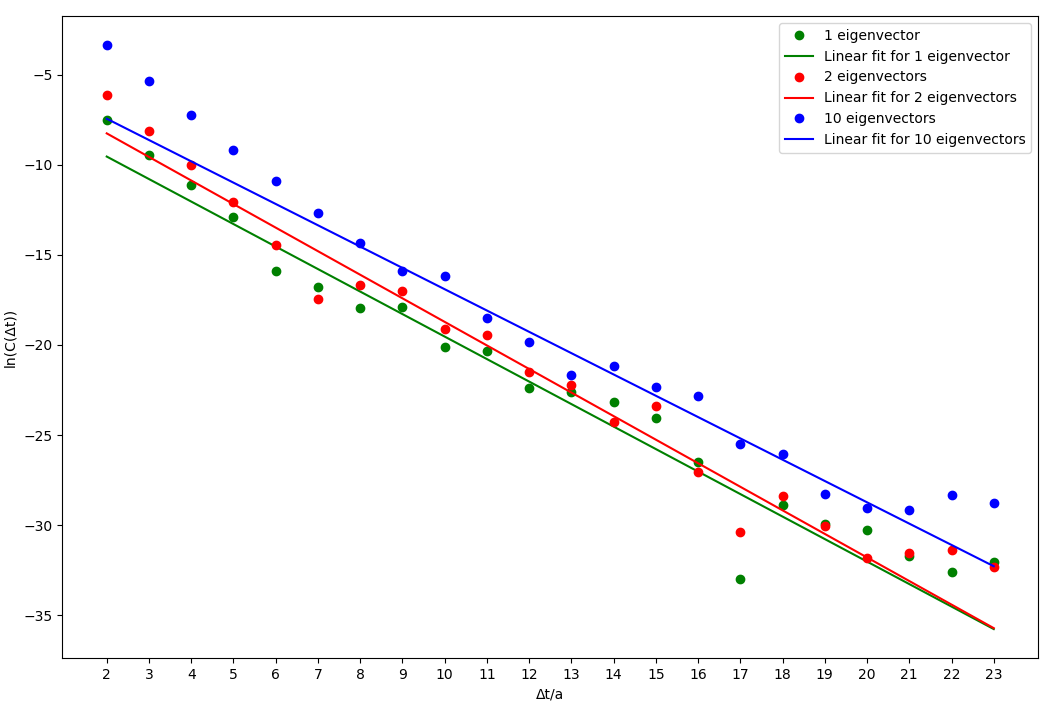
\includegraphics[width=1\textwidth]{images/1_2_10_log.png}
        \caption{Logarithmic results for 1, 2, 5 and 10 eigenvectors}
        \label{1_2_5_10_evs_log}
    \end{figure}
    
    \subsubsection{Details for 10 eigenvectors}
    In this section the result for a simulation with $N = 10$ will be presented and all necessary steps discussed. In figure \ref{10_evs_full} the complete set of results from all 11 configurations can be seen.

    \begin{figure}[H]
        \centering
        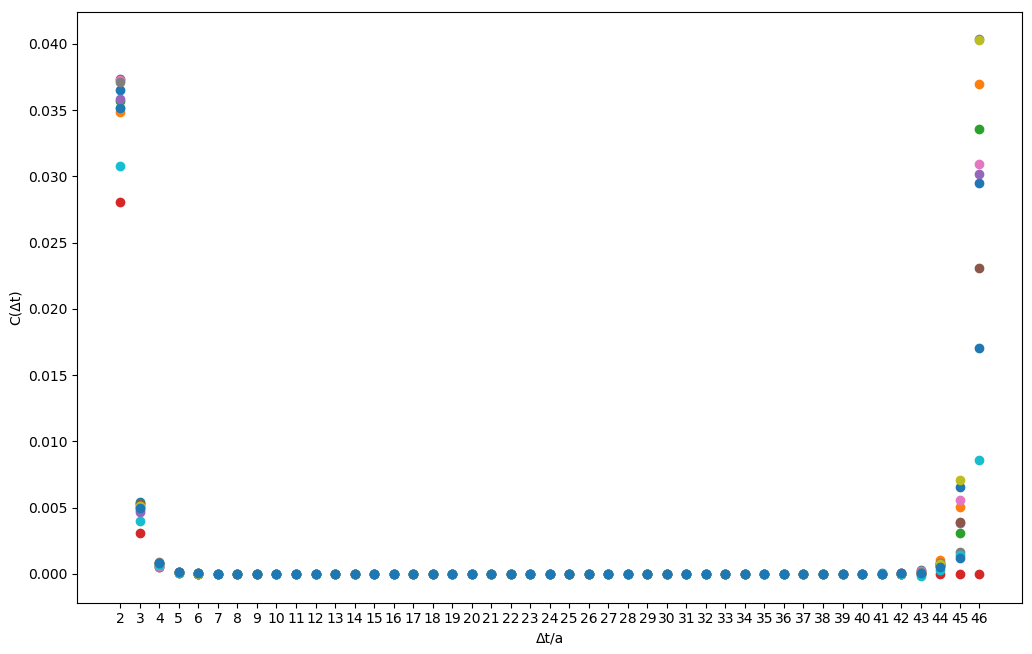
\includegraphics[width=1\textwidth]{images/10_ev_full.png} % first figure itself
        \caption{Data from all 11 configurations for 10 eigenvectors, every color represents one configuration}
        \label{10_evs_full}
    \end{figure}
    
    In figure \ref{10_evs_log} one can see the logarithmic fit to the mean values of all 11 configurations and the data points used for fitting. An important observation is the linear region roughly between $\Delta t = 8$ and $\Delta t = 19$ while the other parts of this graph diveates from the linear path.
    
    \begin{figure}[H]
        \centering
        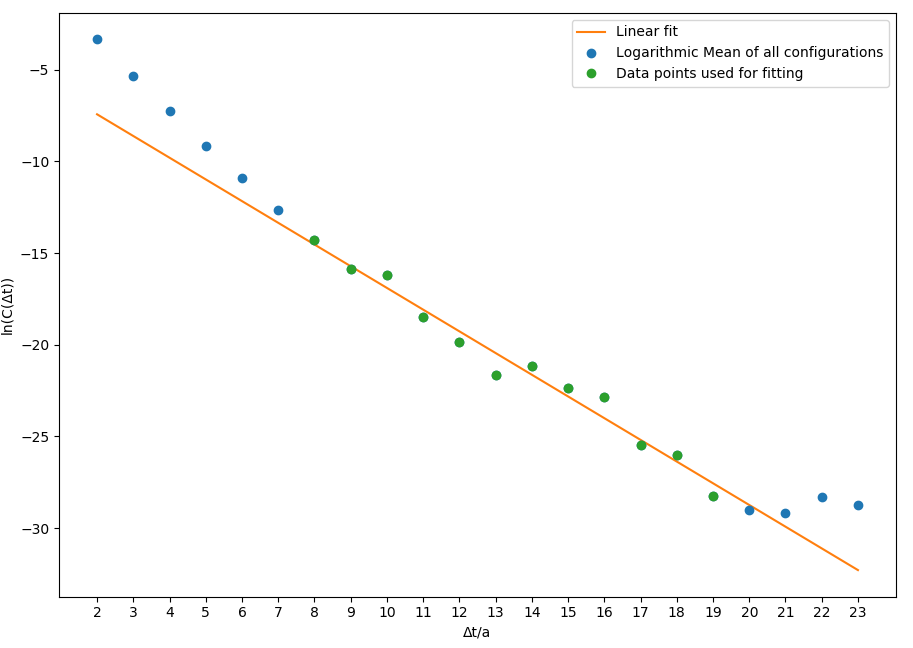
\includegraphics[width=1\textwidth]{images/10_log_fit.png}
        \caption{Logarithmic result for 10 eigenvectors}
        \label{10_evs_log}
    \end{figure}